To simulate communication between the user and the ideal smartwatch application (acting as the smart pacer), can be established an MQTT session. This setup allows the user to send data to the smartwatch app, which processes the information (by running the RunnerEnv) and provides feedback, including suggested actions to take during the training.

\subsection{Run the simulation}\label{subsec:start-application}
The application is designed to run in a terminal environment, that can be done by exectuing the \texttt{main.py} file, which is the entry point of the application.
After starting it, the terminal will prompt for information about the athlete to find the closest archetype profile, as defined in sec.~\ref{sec:methodology}. The user will be asked to provide the necessary details to build the athlete profile, as explained in sec.~\ref{sec:settings}. 
After that, the user selects the type of workout to perform, and finally, the application asks whether to create an MQTT session to simulate communication with the smartwatch application. 
All these steps are shown in the fig.~\ref{fig:main_question} and~\ref{fig:recap_main}.

\begin{figure}[htbp]
    \centering
    \begin{subfigure}[t]{0.52\textwidth}
      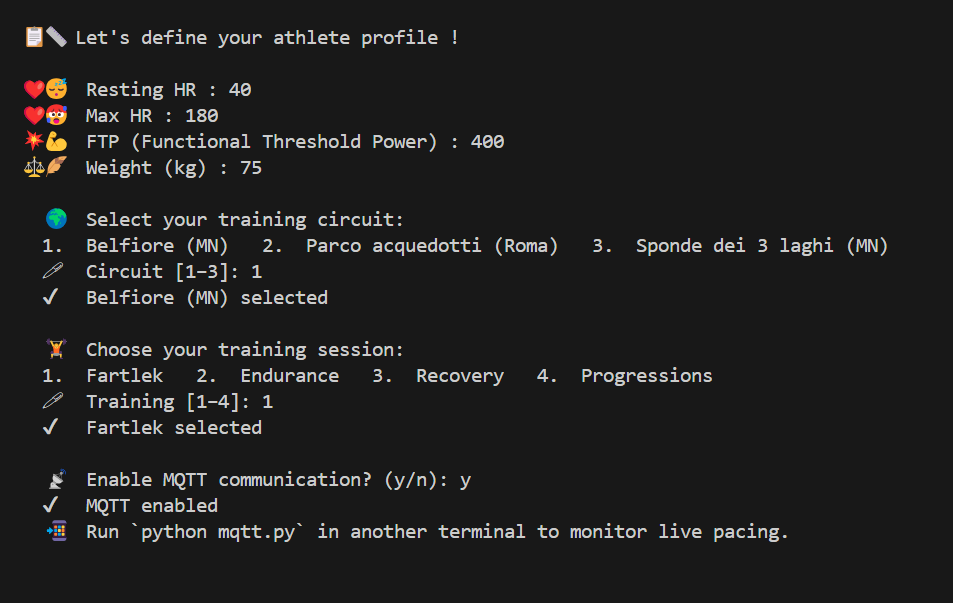
\includegraphics[width=\textwidth]{images/question_main.png}
      \caption{Question about the athlete's parameters in order to choose the right athlete archetype}
      \label{fig:main_question}
    \end{subfigure}
    \begin{subfigure}[t]{0.45\textwidth}
      \centering
      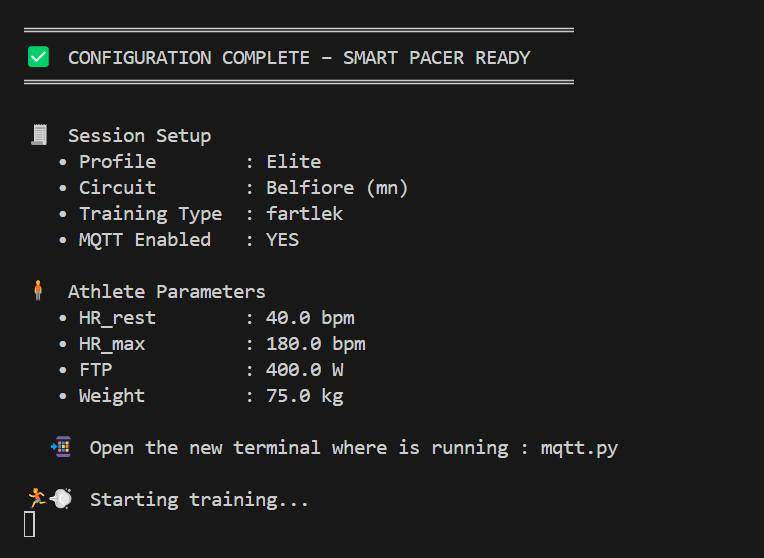
\includegraphics[width=\textwidth]{images/recap_main.png}
      \caption{Recap provided by the application after the user has provided their parameters.}
      \label{fig:recap_main}
    \end{subfigure}
    
    \caption{Messages shown in the terminal when starting the application.}
  \end{figure}



If the MQTT session is not created, the application will run the simulation and provide the results inside the folder \texttt{training\_logs}, with all the information recorded second by second. 

The user can then analyze the results and see how the smart pacer would have guided them through the training session.

\subsection{MQTT Messages}\label{subsec:mqtt-messages}
The communication occurs over the topic \texttt{smartpacer/action} using the public broker
\texttt{broker.emqx.io}. The smart pacer publishes messages at a frequency of 1~Hz, meaning it sends
updates every second during the workout session. This frequency is chosen to provide timely feedback
to the athlete, allowing them to adjust their pace and actions in real-time based on the smart pacer's
suggestions. The payload of each MQTT message is a JSON object containing the following fields:
\begin{itemize}
  \item \texttt{second}: the current second of the workout;
  \item \texttt{phase}: the current phase of the workout;
  \item \texttt{fatigue}: the athlete's current fatigue level;
  \item \texttt{action}: the action suggested by the smart pacer, which can be one of
    \emph{accelerate}, \emph{hold}, or \emph{ease}.
\end{itemize}

Each field is represented as a string, accompanied by a relevant emoji to enhance the user experience.
An example of messages is shown in figure~\ref{fig:mqtt_message_example_emoji}.

\begin{figure}[htbp]
    \centering
    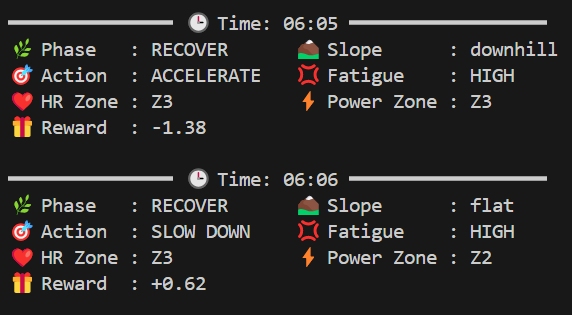
\includegraphics[width=0.90\textwidth]{images/mqtt_message.png}
    \caption{Example of an MQTT message with emojis.}
    \label{fig:mqtt_message_example_emoji}
\end{figure}

